\documentclass[11pt,twoside]{report}
\usepackage{preamble}
\graphicspath{{../img/ch7/}}
\setcounter{chapter}{6}

\begin{document}

\chapter{Collective Behaviour of Mutant Zebrafish}
\label{chapter:fish_mutation}

\section{Introduction}

%Understanding the behaviours of zebrafish is not only intellectually fulfilling, but it is also useful. Appreciating the stochastic nature of the animal behaviours, the detailed knowledge of zebrafish would enable us identify the behavioural differences among different groups, without being mislead by the randomness of animal behaviours.

In this chapter, the methods developed in previous chapters will be applied to study the behavioural change of zebrafish when they carry mutations in genes relevant to human disease. The idea is to use the behavioural feature as a probe, so that we could test the functions of different genes.
Such idea was implemented by the pioneering work from \citeauthor{tang2020}, who tested the behaviours of different fish groups with different genetic modifications \cite{tang2020}. Even though the massive screening process could pick up different features of different genetic mutations, there is little explanation for the observations.

Instead of screening many different genes, we will take a different approach, and only focus on one particular gene in this chapter, the \emph{col11a2} gene. This gene is responsible for the production of an alpha chain of type XI collagen \cite{lawrence2018}.
Mutations to Col11a2 (as well as to Type II and Type IX collagen) are associated with Stickler syndrome. Stickler syndrome is characterised by hearing loss, problems with vision, and progressive changes to the skeleton which result in severe early onset osteoarthritis \cite{vikkula1995, jakkula2005}.
For zebrafish, such mutation is also found to cause premature osteoarthritis \cite{lawrence2018}.
%It is expected, that the interruption of the development of bones and the cartilage would change the behaviour of the fish.
Here we hypothesise that changes to the skeleton, or to visual and auditory perception would lead to changes to swimming behaviour, either through increased joint stiffness or a failure to correctly perceive their position in the water.
This expectation is supported by the reported correlation between swimming performance and the development of bones \cite{fontaine2008} and cartilage \cite{tseng2021}.

Observing, analysing, and modelling the 3D swimming behaviour from both the mutant fish, and the wildtype (\gls{wt}) fish, we studied the behavioural differences caused by the col11a2 mutation. Notably, the mutant fish have a significantly longer orientational relaxation time ($\tau_\mathbf{o}$ in Eq.~\ref{eq:tau}). And the slow reorientation of the mutant fish leads to a longer persistence length, since the speed of both kinds (the mutant and the wildtype) are similar. Collectively, the mutant fish exhibit higher polarisation value, which can be explained by the dynamical model in chapter~\ref{chapter:fish_model}. Our analysis provided the behavioural feature of the mutant fish, and provide a direct link between the microscopic feature of the fish to their corresponding collective behaviour.
The linkage is remarkable, because it bridges the gap between the biological feature of the fish and the collective behaviour of the group, under the framework of active matter physics.
%from the single fish property to the corresponding collective behaviour is interesting from the perspective of physicists. Such result suggests that the collective motion of both the wt fish and the {\mf} follow the same physical laws, and the effect of the genetic modification is, effectively, a change of the parameter. 


\section{Method}

\subsection{Mutant Fish}

The {\mf} have a nonsense mutation, i.e. in the mutants the Coll1a2 protein is no longer produced. The mutant fish were obtained from European Zebrafish Resource Centre and bred in the fish facility in the university of Bristol \cite{lawrence2018}. Two generations of mutant fish were crossed by Elizabeth A. Lawrence and Erika Kague respectively from the university of Bristol. The wildtype zebrafish were also crossed and bred in the same time, so that the two groups sharing the same growth condition can be compared. For each generation, the number of wt fish is $\sim$ 50, and the number of mutant fish is $\sim$ 30. 

The two different generations of ``mutant + wildtype'' combinations, crossed at different time points, exhibits consistent behavioural features. The fish were observed when they were 40 days post fertilisation (\gls{dpf}), by which point they are relatively skeletally mature. We carried out the observation repeatedly, until the fish were about 120 dpf.

\subsection{Experiments and Analysis}

Both the mutant fish and the wildtype fish were kept in aquarium tanks in a separate room, without the observation equipment. The husbandry of the fish is introduced in section~\ref{section:apprautus_2d}.

For the one-fish experiment, we randomly took 10 fish from their living tank, to the observation room, and recorded the movement of each fish individually for 10 minutes at a frequency of 15 frames per second. We then circulate the water in the observation tank for 5 minutes to remove possible olfactory responses \cite{kalueff2013}, then started recording for another fish. We carried out the experiment for the two generations of the mutant and wildtype fish, therefore tested 40 fish in total.

\marginpar{
\centering
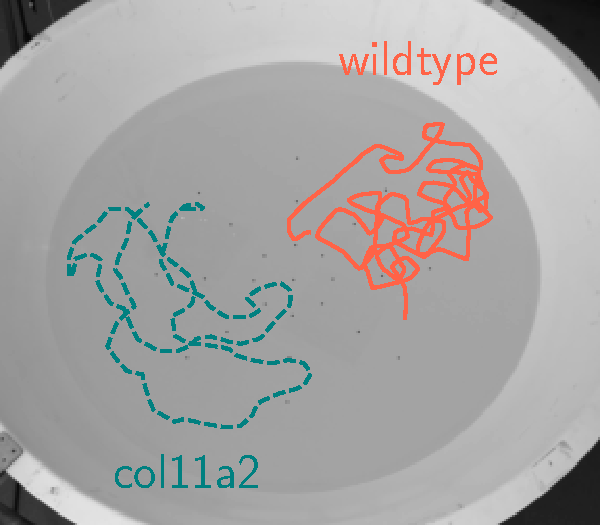
\includegraphics[width=\marginparwidth]{mutant-traj}
\captionof{figure}[Typical trajectories of the col11a2 mutant zebrafish and the wildtype zebrafish]{
	Typical trajectories of the col11a2 mutant zebrafish and the wildtype zebrafish
}
\label{fig:mutant-trajs}
}

For the many-fish experiments, we randomly selected 25 fish, and transferred them to the observation tank. We waited 10 minutes for the group to get familiar with the new environment, and then started recording their movement. We carried out the experiment for the two different generations, and we tested 4 groups, 100 fish in total.

The 3D fish tracking apprautus, introduced in chapter~\ref{chapter:fish_3d}, was used to record the 3D coordinates of the fish.
These coordinates were then linked into trajectories following the methods discussed in chapter~\ref{chapter:fish_analysis}. The trajectories were analysed following the methods in chapter~\ref{chapter:fish_analysis}, yielding the results that could be fitted with the modified Vicsek model with inertia (chapter~\ref{chapter:fish_model}).


\section{The Behaviour of A Single Mutant Fish}
\label{section:mutant-1-fish}


The movement of one single fish differs significantly between the wt fish and the {\mf}, as shown in Fig.~\ref{fig:mutant-1}.
For all the different fish individuals, they tend to move near the surface of the tank, as seen in Fig.~\ref{fig:mutant-1} (a).
Comparing with the {\mf}, the wt fish prefer the bottom of the tank, as shown in Fig.~\ref{fig:mutant-1} (c).
Besides the spatial distribution, the wt fish frequent stops swimming in the tank, indicated by the peak around 0 mm/s in the speed distribution (Fig.~\ref{fig:mutant-1} (d)).
However, the wildtype fish also have a longer tail in the speed distribution, meaning they are more likely to enter the high speed state (speed $>$ 300 mm/s).


A notable difference between the wt fish and mutant fish is the dynamics of the orientation.
The {\mf} took a significantly longer time to change their directions, indicated by the auto correlation function of the moving direction (\gls{cot}, Eq.~\ref{eq:acf}) of the fish.
The results are shown in Fig.~\ref{fig:mutant-1} (e).
By fitting the ACFs with an exponential function (Eq.~\ref{eq:tau}), we obtained the characteristic reorientation timescale of the wt fish (0.38s) and {\mf} (0.8s). Visually, the slow re-orientation of the {\mf} leads to a smoother trajectory, while the trajectory of the wt fish appeared to be more zigzag. These characteristic trajectory shapes were shown in Fig.~\ref{fig:mutant-trajs}. 
The slower re-orientation of the mutant fish might be attributed to their altered skeletal phenotype in which joints are abnormal \cite{lawrence2018}. But more work is needed to prove this causality.


\begin{SCfigure}
  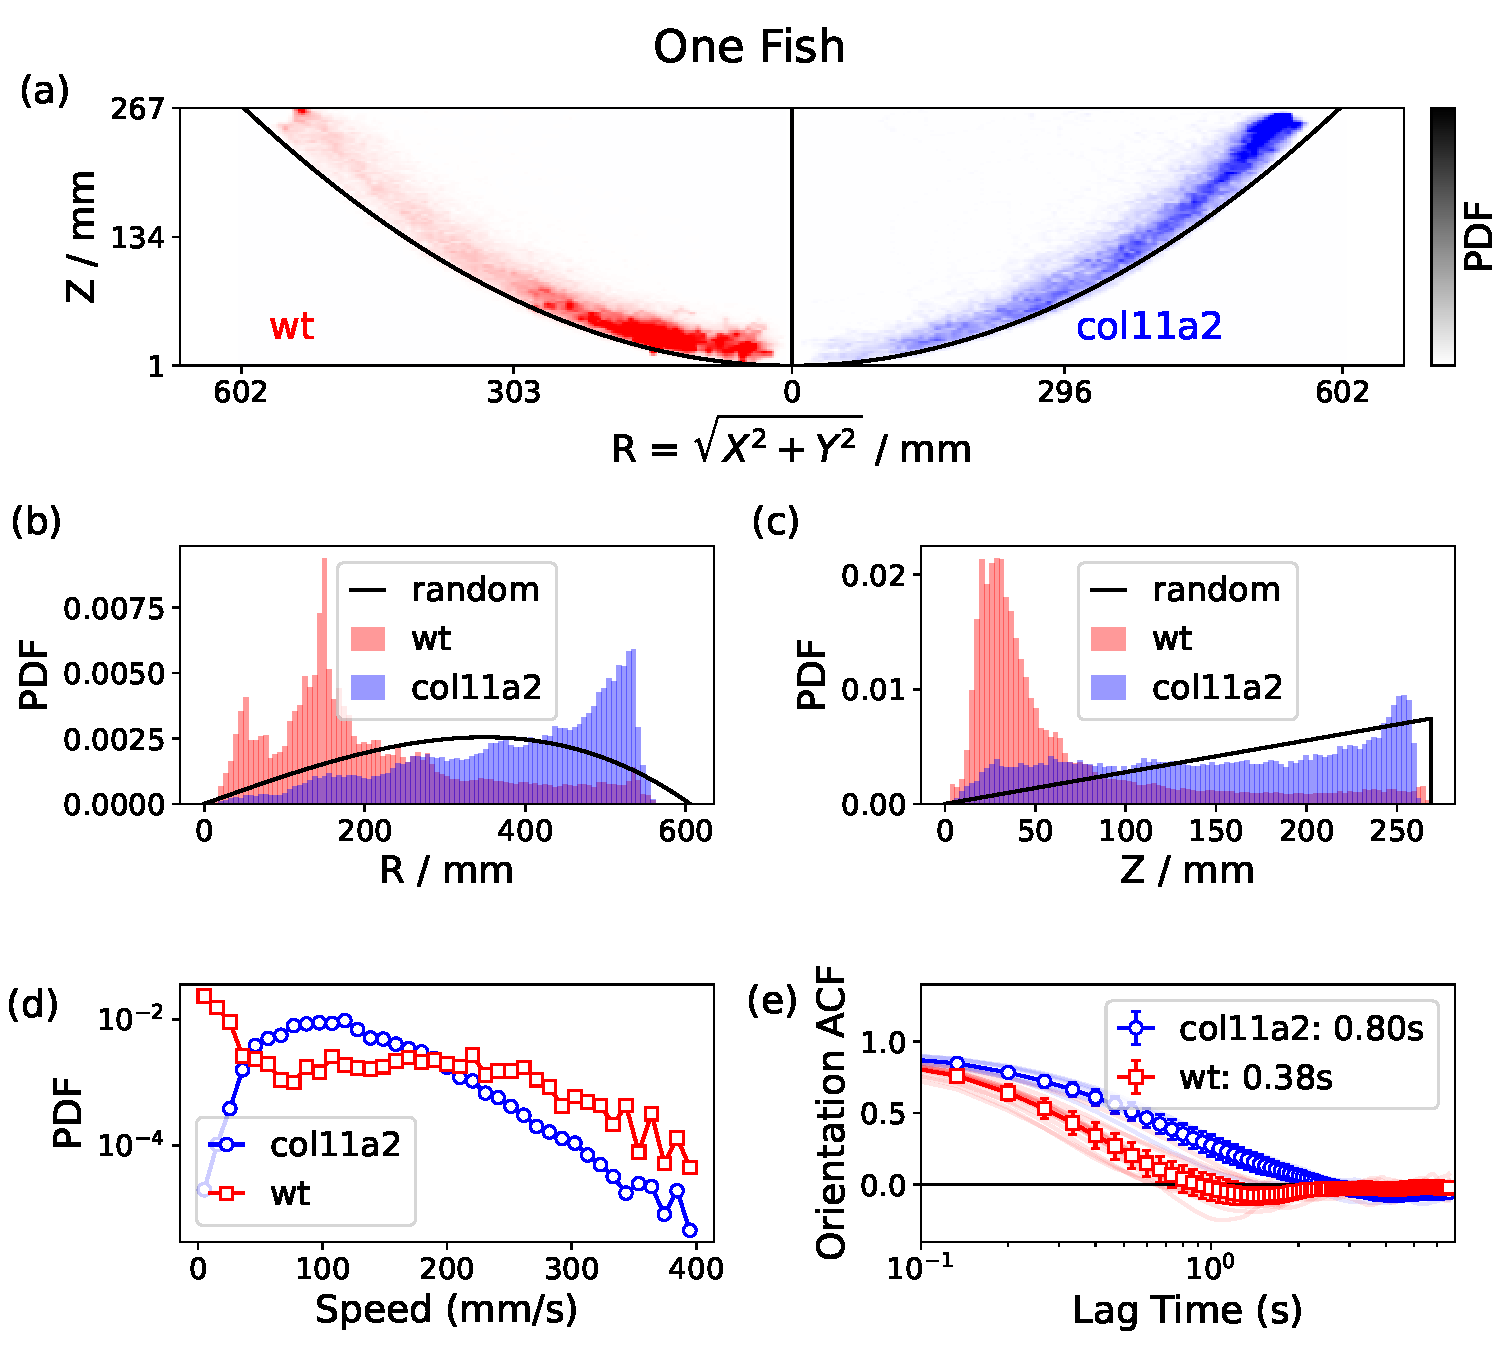
\includegraphics[width=\linewidth]{behaviour-1}
  \caption[The behaviour of one mutant fish and one wildtype fish]{
  	The behaviour of 1 mutant fish and 1 wt fish.
  	(a) The joint probability density function (PDF) of the 2D radius and the Z coordinate of the fish.
  	(b) The marginal PDF of the 2D radius. 
  	(c) The PDF of the height of the fish.
  	(d) The distribution of speed of the fish.
  	(e) The average auto-correlation function of the orientation of the fish.
  	The solid line in (a) presents the outline of the observation tank. The solid lines in (b) and (c) indicate the corresponding distributions of ideal gas in the tank.
  }
\label{fig:mutant-1}
\end{SCfigure}



It is important to point out, that we took extra care for the calculation of the relaxation time, since the re-orientation process of the fish can be affected by extrinsic factors.
For instance, the directional change of the non-moving fish will be dominated by the tracking error, and the fish in the bottom of the tank will be forced to change direction more frequently, because the otherwise ballistic motion will be interrupted by the tank.
To exclude these extrinsic effects, we excluded the non-moving time points in the trajectories (speed $< 50$ mm/s), and focused only on a specific hight region ($50 \mathrm{mm} < z < 150 \mathrm{mm}$) during the calculation of the ACF\@.
The choice of the speed threshold or the height region will not affect the conclusion, but will change the numerical value of these time scales.


In summary, we find three significant difference between the wt fish and the {\mf}.
The wt fish prefer the bottom of the tank, and the wt fish tend to stop swimming during the observation.
The {\mf} however takes much longer time to change their moving directions, presenting a smoother trajectories over time (Fig.~\ref{fig:mutant-trajs}).
These features were robust, as we repeated the experiment by crossing two new groups of wt fish and the {\mf}, and obtained results leading to the exact same conclusions.



\section{The Behaviour of Many Mutant Fish}

In addition to the one fish experiment, we also observed a group ($n = 25$) of wt fish and {\mf}, and analysed their behaviours.
Visually, the {\mf} are more likely to swim together, while the movement of the wildtype fish seemed more random. The typical trajectories of 25 wt fish and 25 {\mf} are shown in Fig.~\ref{fig:traj-mutant}. Where the trajectories captured by the cameras were presented in Fig.~\ref{fig:traj-mutant} (a) and (b), whose corresponding 3D trajectories were shown in Fig.~\ref{fig:traj-mutant} (c) and (d), respectively.

\begin{SCfigure}
  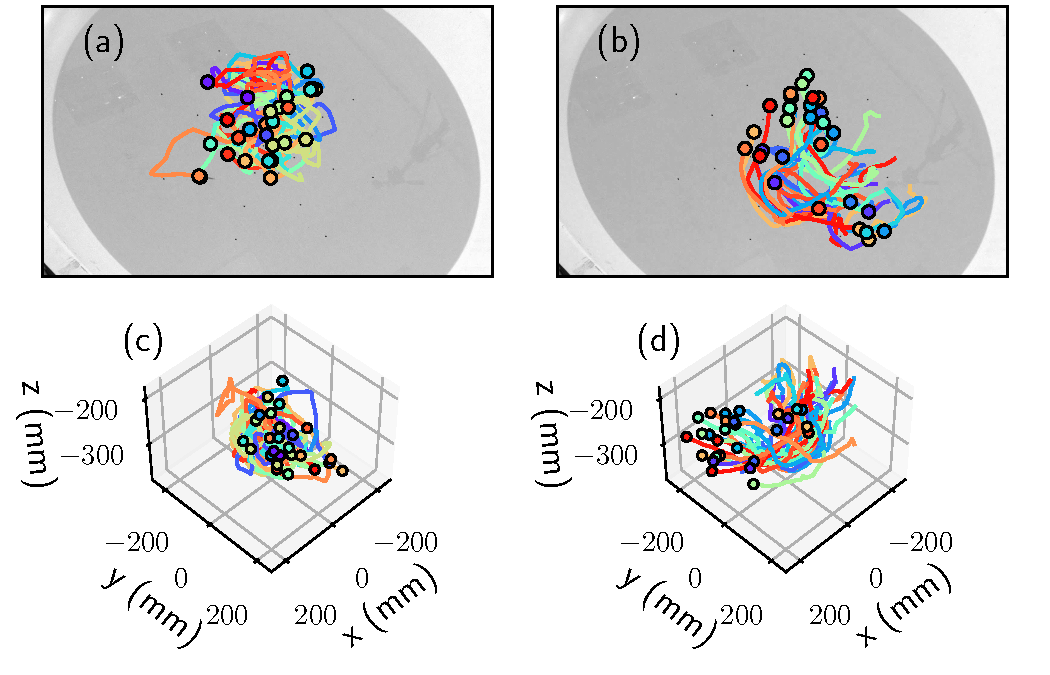
\includegraphics[width=\linewidth]{traj-mutant}
  \caption[The trajectories of 25 wildtype zebrafish and {\mf}]{
  	The trajectories of 25 wildtype zebrafish and {\mf}.
  	(a) The trajectories of wildtype zebrafish projected onto a camera in 5s.
  	(b) The trajectories of \emph{col11a2} zebrafish projected onto a camera in 5s.
  	(c) The 3D trajectories of wildtype zebrafish in 5s.
  	(d) The 3D trajectories of \emph{col11a2} zebrafish in 5s.
  }
  \label{fig:traj-mutant}
\end{SCfigure}


\subsection{The Behavioural Features of {\mf}}
\label{section:mutant-feature-many}


All of the behavioural features of the mutant fish, summarised in section~\ref{section:mutant-1-fish}, were also observed in the 25 fish experiment, as shown in Fig.~\ref{fig:mutant-25}.
Namely, the wt fish tend to distribute at the bottom of the tank (Fig.~\ref{fig:mutant-25} (a) and (c)), and these fish also tend to stop swimming, leading to a peak around 0 mm/s in the distribution of the speed values (Fig.~\ref{fig:mutant-25} (d)).
In contrast, the {\mf} present different spatial distribution and speed distribution, as the {\mf} were more likely to stay on the top of the water, and tend to maintain a moderate swimming speed.

\begin{SCfigure}
	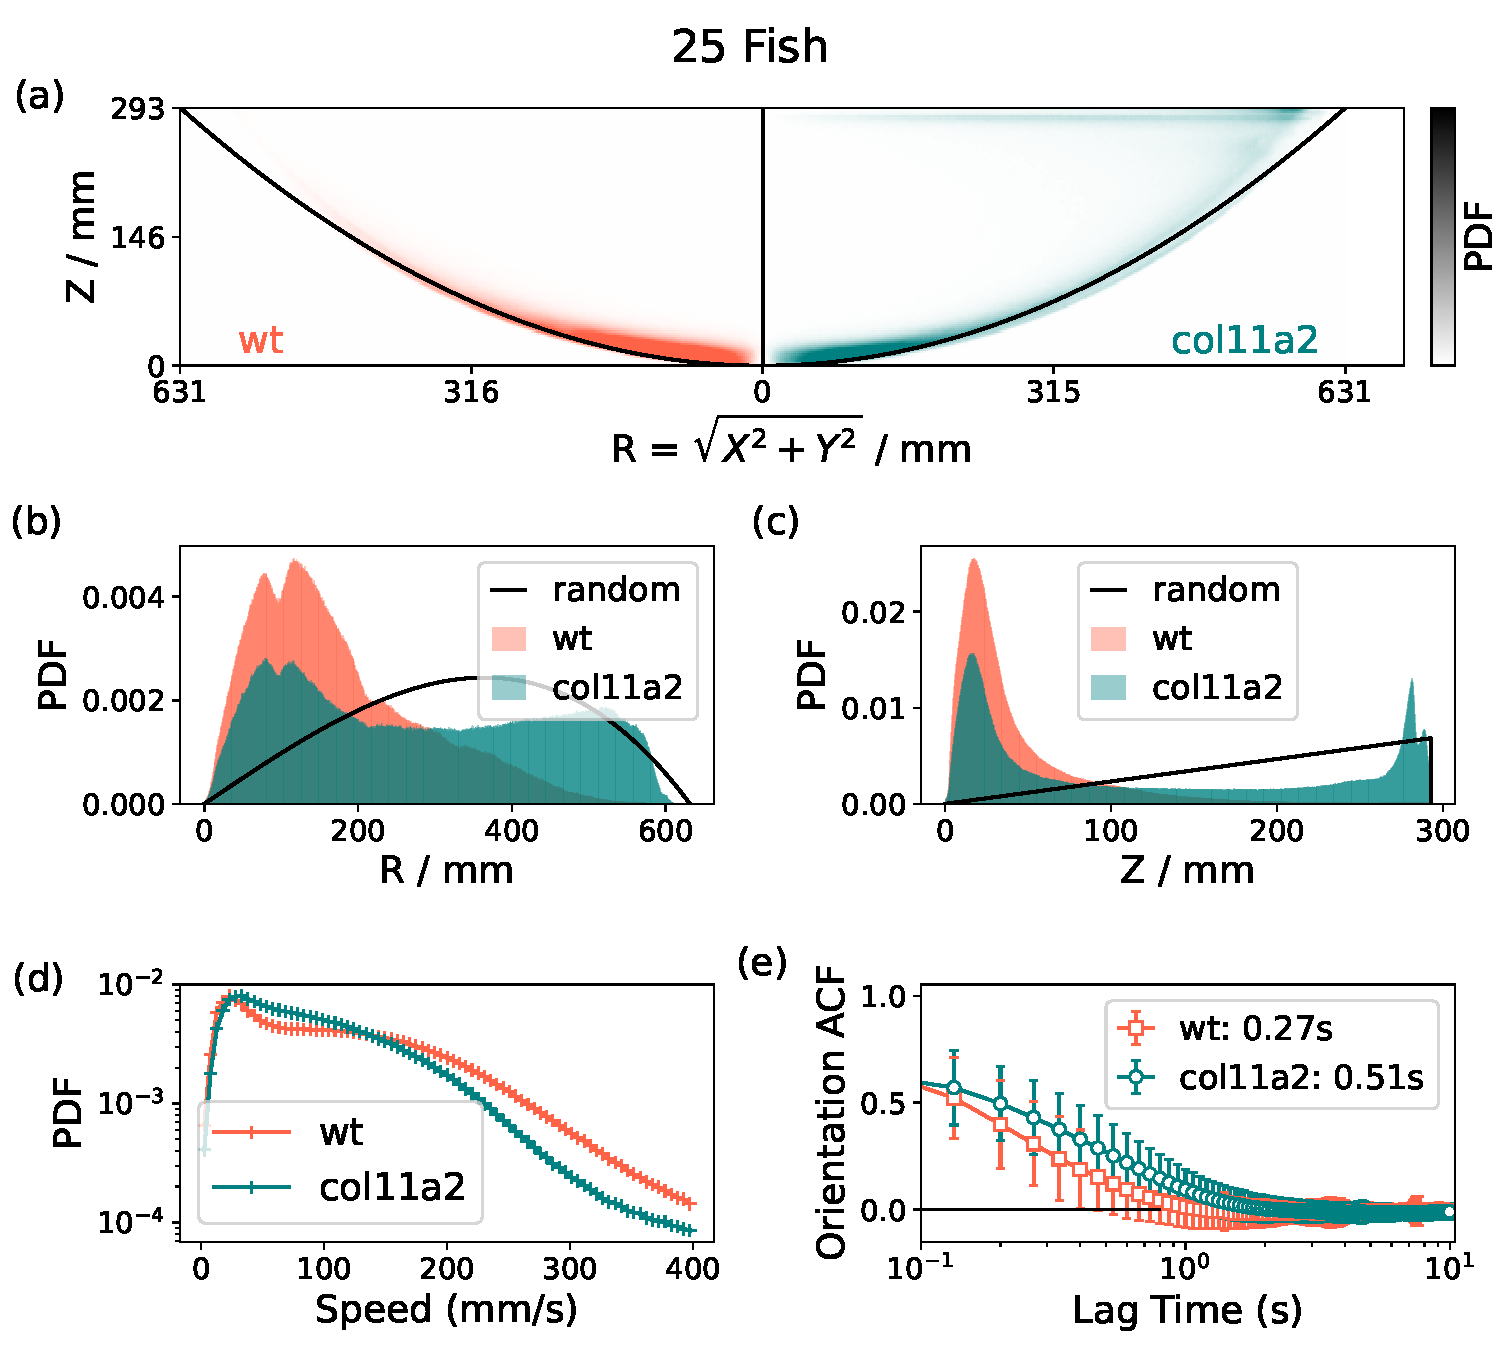
\includegraphics[width=\linewidth]{behaviour-25}
	\caption[The Collective Behaviour of 25 wt fish and {\mf}.]{
        The Collective Behaviour of 25 wt fish and {\mf}.
        (a) The joint probability distribution of the latitude radius ($r$) and the height ($z$) of the wt fish (left) and the {\mf} (right).
        (b) The probability density function of the latitude radius ($r$).
        (c) The probability density function of the hight ($z$).
        The solid line in (b) and (c) represents the analytical distribution of uniformly random points.
        (d) The probability distribution of the speed.
        (e) The averaged auto-correlation function of the fish orientation.
    }
\label{fig:mutant-25}
\end{SCfigure}


The different orientational relaxation time ($\tau_\mathbf{o}$) values, as illustrated in Fig.~\ref{fig:mutant-25} (e), were also observed in the many-fish experiment.
The {\mf} have a typical value of $\tau_\mathbf{o} = 0.5s$, while the wildtype fish have a typical relaxation time of $\tau_\mathbf{o} = 0.27s$.
The standard deviation of the ACFs from the 25-fish experiments are larger, comparing with the single fish experiment.
This is because we repeated the observation multiple times. And the fish gradually grew during this period. In addition, the repeated exposure to the experimental environments might also change the behaviour of the fish \cite{macgregor2021}. Nevertheless, the different orientational relaxation time values for the {\mf} and wt fish were repeatedly observed, being a robust behavioural feature.



\subsection{The Changing States of {\mf}}
\label{section:change-states-mutant}

The macroscopic states of 25 zebrafish change over time, like the scenario presented in section~\ref{section:change-states-3d} and \ref{section:change-states-2d}. These changing states of wildtype fish were plotted in Fig.~\ref{fig:states-wt}. Figure~\ref{fig:states-wt} (a) shows the ACFs of the polarisation (\gls{pol}), the speed (\gls{spd}), as well as the nearest neighbour distance (\gls{lnn}). Again, we observed the separated timescales, where the relaxation of orientation caused the initial decay of the ACFs, followed by a second decay that indicates the relaxation of the density. 

We segmented the observed trajectories into short segments, whose duration values were 120 seconds, indicated by the vertical bar ``Average Window'' in Fig.~\ref{fig:states-wt} (a). The statistical analysis on these segments revealed the fluctuating behaviour of 25 wildtype fish. Figure~\ref{fig:states-wt} (b) shows the changing $C_\mathbf{o}(t)$ functions of the wt fish, which lead to the fluctuating $\tau_\mathbf{o}$ values in Fig.~\ref{fig:states-wt} (d). Similarly, the fish group also presents varying degree of cohesion, captured by the effective attraction \gls{attr} in Fig.~\ref{fig:states-wt} (d). The changing cohesion levels are also obvious in the radial distribution function of the fish shown in Fig.~\ref{fig:states-wt} (c).

These changing states are visually correlated, like the results from section~\ref{section:change-states-3d} and \ref{section:change-states-2d}. Importantly, the correlations are consistent. The dynamical quantities ($\Phi$ and $v$) are correlated, while the structural quantities ($l_\mathrm{nn}$ and $\epsilon$) are correlated. The orientational relaxation time ($\tau_\mathbf{o}$) correlates with the structural quantities, where the fish exhibited slower reorientation when they were less cohesive. The changing relaxation time values could be explained by the short range repulsive interaction of the fish (section~\ref{section:change-states-3d}).

\begin{SCfigure}
	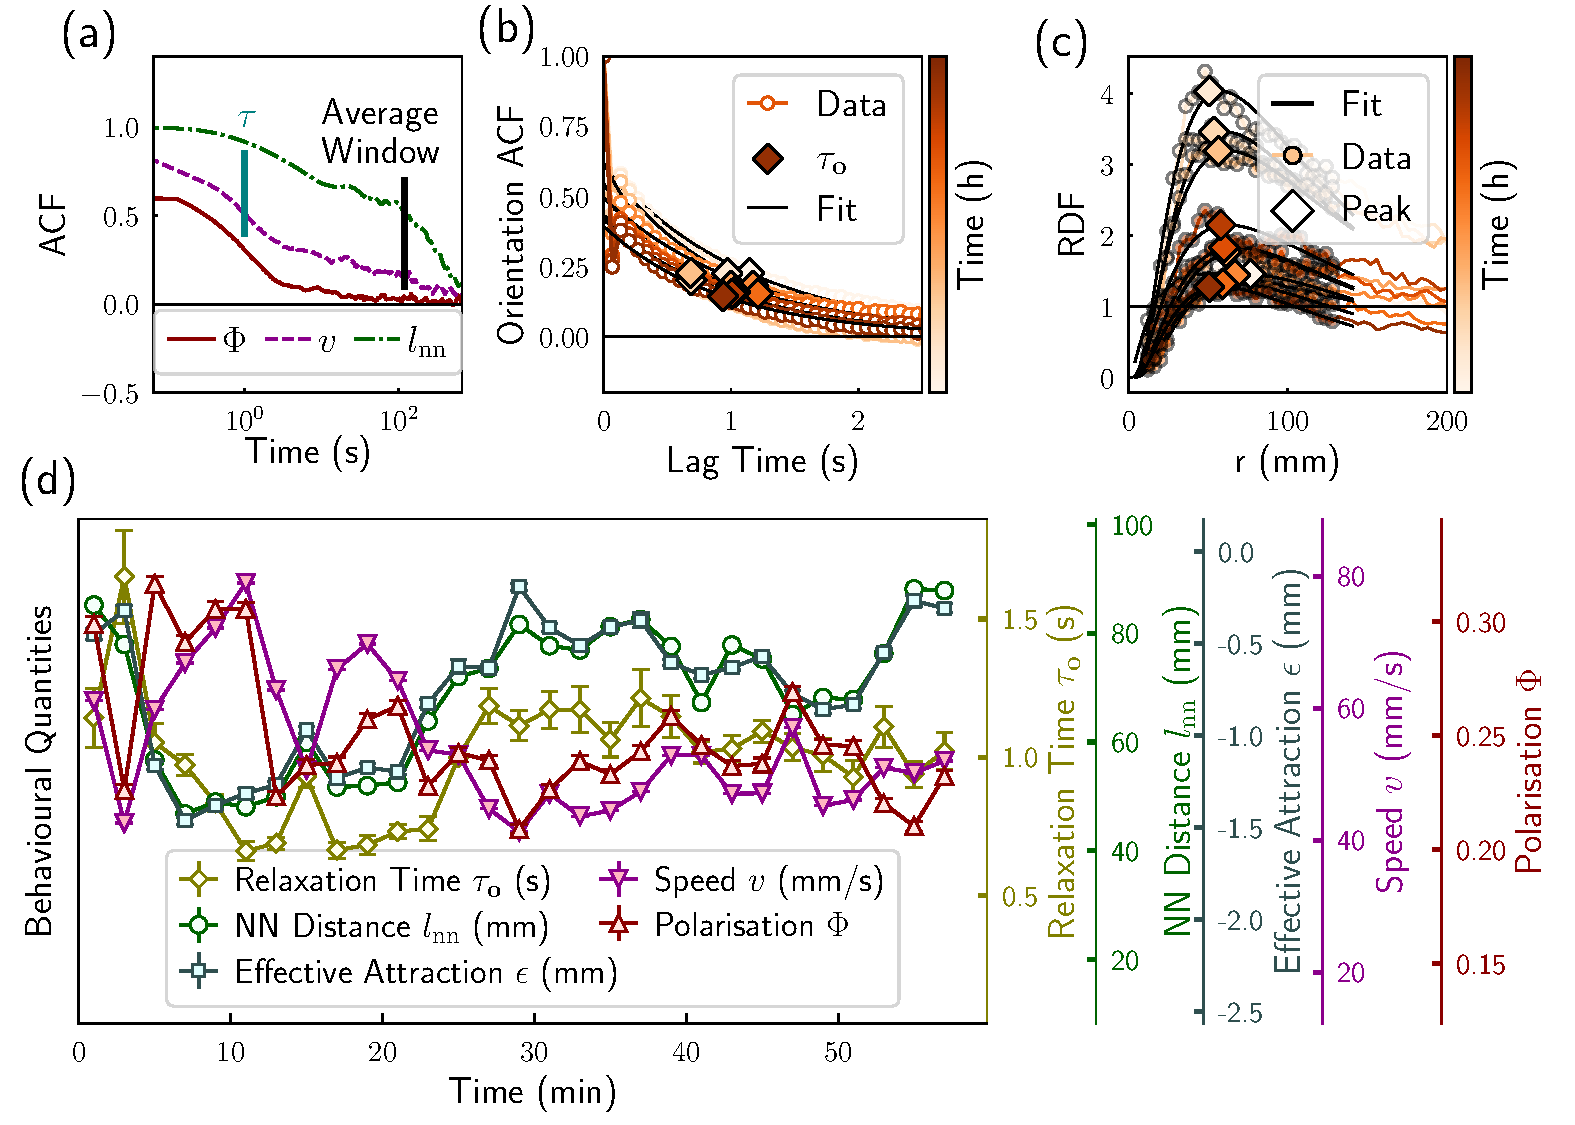
\includegraphics[width=\linewidth]{states-wt}
	\caption[The changing states of 25 wt zebrafish]{
        The Collective Behaviour of 25 wt zebrafish.
        (a) The ACFs of the polarisation ($\Phi$), the speed ($v$), and the nearest neighbour distance ($l_\mathrm{nn}$). The first decay corresponds to the relaxation of the orientation, and the second decay is taken as the average window where the long  trajectories were segmented into.
        (b) The ACFs of the orientations ($C_\mathbf{o}(t)$) of the fish at different time points.
        (c) The radial distribution function (RDF, the $g(r)$) of the fish group at different time points. The heights of the peaks are linked to the effective attraction ($\epsilon$) of the fish.
        (d) The changing states of the fish captured by the orientational relaxation time ($\tau_\mathbf{o}$), the speed ($v$), the polarisation ($\Phi$), the nearest neighbour distance ($l_\mathrm{nn}$), and the effective attraction ($\epsilon$).
    }
\label{fig:states-wt}
\end{SCfigure}


For 25 {\mf}, we also observed their changing states in a very similar fashion, as shown in Fig.~\ref{fig:states-col11a2}. One notable difference between the wt fish and the {\mf} is the ACF of the nearest neighbour distance. Specifically, the first decay reached to a value close to 0.3, meaning the system will forget about its current $l_\mathrm{nn}$ quicker than the wt fish. For consistency, we still applied the duration of 120 seconds to segment the trajectories of the {\mf} temporally, and analyse the evolving states.

The orientational relaxation time of the {\mf} is significantly longer than that of the wt fish. The wildtype fish have a $\tau_\mathbf{o}$ value around 1s, while the {\mf} have a $\tau_\mathbf{o}$ value around 2s. These two values here are larger than that from section~\ref{section:mutant-feature-many}, because the data presented in Fig.~\ref{fig:states-wt} and \ref{fig:states-col11a2} were obtained when the fish were 40 dpf. In contrast, the results presented in section~\ref{section:mutant-feature-many} are the average of different experiments during which the fish were aging.

In addition, the {\mf} appear more cohesive than the wt fish, characterised by the high peaks in the RDF of the {\mf}. This feature can not be captured by conventional methods such as the nearest neighbour distance. In fact, the {\mf} have a larger $l_\mathrm{nn}$ values compared with the wildtype counterpart. However, the {\mf} are more cohesive because the are more likely to have a pairwise distance around 10 cm. It is this probability that captured the cohesive feature, rather than the physical length scale. Even though these two are normally correlated.


\begin{SCfigure}
	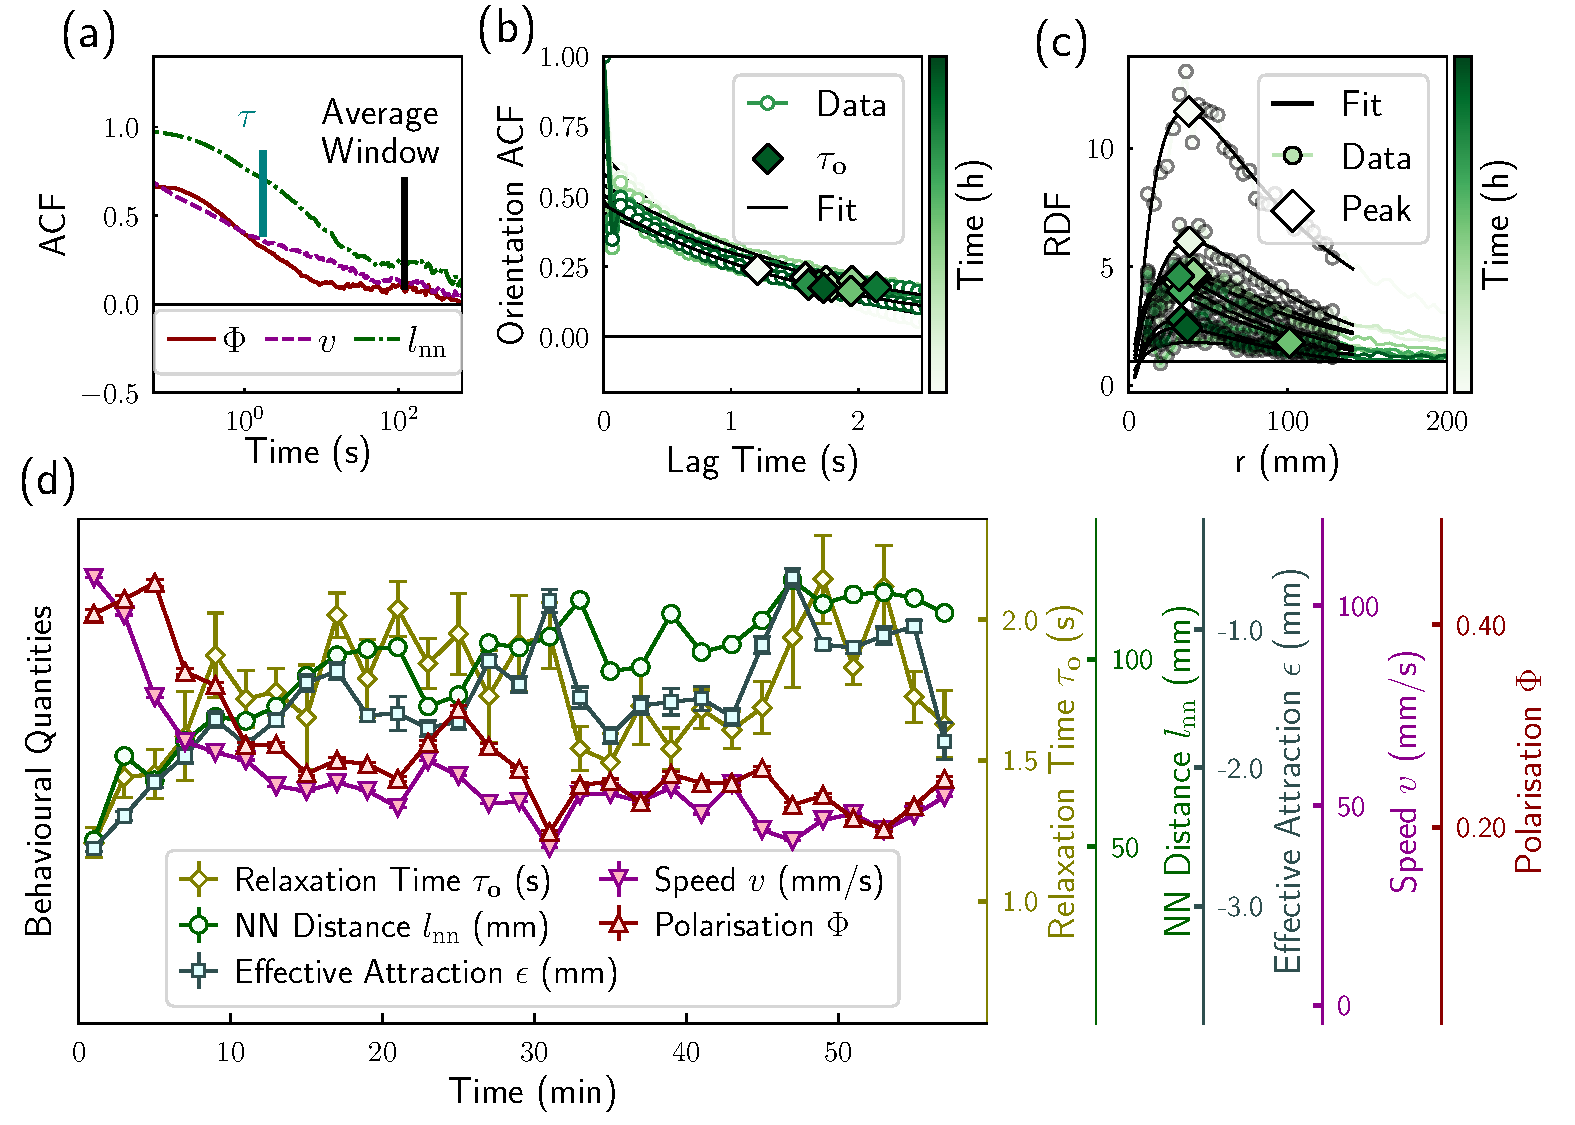
\includegraphics[width=\linewidth]{states-col11a2}
	\caption[The changing states of 25 col11a2 zebrafish]{
        The Collective Behaviour of 25 col11a2 zebrafish.
        (a) The ACFs of the polarisation ($\Phi$), the speed ($v$), and the nearest neighbour distance ($l_\mathrm{nn}$). The first decay corresponds to the relaxation of the orientation, and the second decay is taken as the average window where the long  trajectories were segmented into.
        (b) The ACFs of the orientations ($C_\mathbf{o}(t)$) of the fish at different time points.
        (c) The radial distribution function (RDF, the $g(r)$) of the fish group at different time points. The heights of the peaks are linked to the effective attraction ($\epsilon$) of the fish.
        (d) The changing states of the fish captured by the orientational relaxation time ($\tau_\mathbf{o}$), the speed ($v$), the polarisation ($\Phi$), the nearest neighbour distance ($l_\mathrm{nn}$), and the effective attraction ($\epsilon$).
    }
\label{fig:states-col11a2}
\end{SCfigure}

\subsection{Modelling the dynamics of {\mf}}

We projected the changing states of the fish onto a ``phase diagram'', spanned by the persistence length (\gls{lp}, Eq.~\ref{eq:lp}) and the nearest neighbour distance ({\dnn}, Eq.~\ref{eq:nnd}). The result was shown in Fig.~\ref{fig:phase-mutant} (a).
Compared to the wt fish, the {\mf} have both larger {\dnn} and $l_p$.
The larger {\dnn} values of the {\mf} might be related from the fact that these mutant fish distribute in the upper location of the tank, where they naturally get larger volume because of the geometry of the tank.
Even though the {\dnn} value of the {\mf} is larger than the wt fish, these mutant fish appear to be more cohesive, as discussed in section~\ref{section:change-states-mutant}.
The larger $l_p$ of the {\mf} is related to the slow re-orientation of the mutant fish, as the persistence length is defined as the product of the speed and the orientational relaxation time.


We observed the behaviour of 25 fish repeatedly, while the fish were growing. As a result, we could also follow the change of the behaviour of these fish over time. The age of the fish was coloured in Fig.~\ref{fig:phase-mutant}. With the growth of the fish, the value of $l_\mathrm{nn}$ decreased for both the wt group and the mutant group.
This indicates that the fish group became more closely packed as they grew from 40 dpf to over 100 dpf. The decreasing $l_\mathrm{nn}$ amongst the zebrafish was also observed by~\citeauthor{buske2011}~\cite{buske2011}.


For the the observed zebrafish, being whether wt or mutant, their reduced persistence length, defined as $\kappa = l_p / l_\text{nn}$, correlates with the polarisation, as shown in Fig.~\ref{fig:phase-mutant} (b).
Such correlation is similar to the results shown in section~\ref{section:universal}, from 50 adult zebrafish.
Among the two groups, the {\mf} have relatively larger $\kappa$ values comparing with the wt fish, hence presenting higher $\Phi$ values.


The relationship between the $\Phi$ and \gls{kappa} can be explained the variation of the Vicsek model with an inertia term (\gls{alpha}, Eq.~\ref{eq:vicsek-inertia}). To fit the experimental data, we changed the value of \gls{eta} from 0.5 to 1.0, while fixing the values of other variables ($v_0=0.1, \rho=0.5, \alpha=0.63$).
These fixed parameters also fits the behaviour of 50 adult zebrafish, except for the value of the density (we set $\rho=1$ for 50 adult fish).
The consistent fit suggests our proposed model, regardless of its simplicity, does capture the essence of the collective behaviour of zebrafish.

Biologically, the reason for the behavioural difference might related to the compromised development of the cartilage, the bones, or the fine mineral stone in the ear of the fish. A careful examination of these intrinsic factors affecting the mutant fish would be the next step, for a more comprehensive understanding of the behaviour, as well as the genetic functions of the col11a2 mutant fish.


 \begin{SCfigure}
  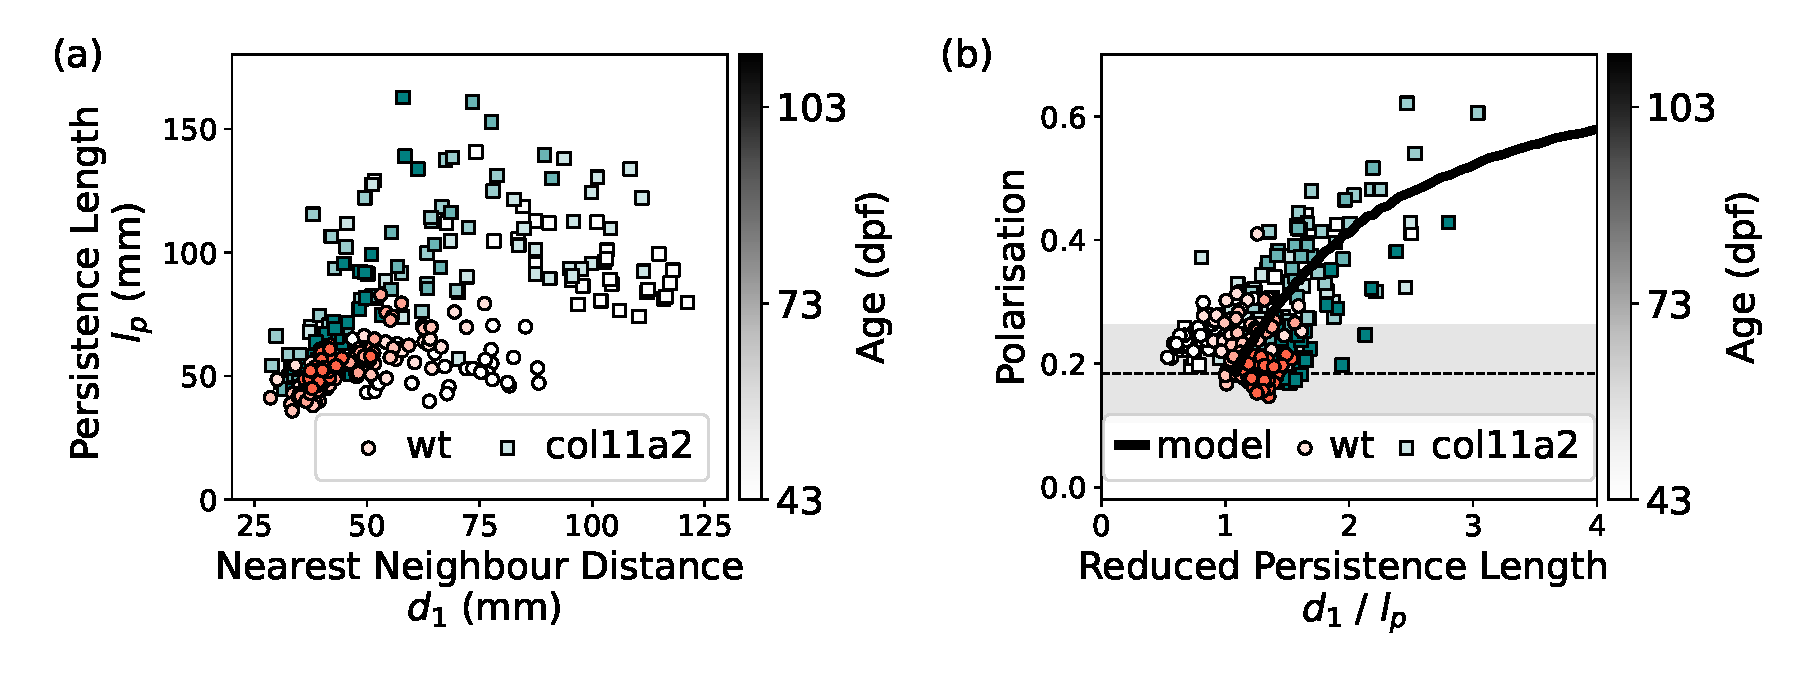
\includegraphics[width=\linewidth]{phase-25}
  \caption[The behaviour of 25 zebrafish described by $l_\mathrm{nn}$ and $l_p$]{
	The behaviour of 25 zebrafish described by $l_\mathrm{nn}$ and $l_p$.
	(a) The changing macroscopic states of the fish projected on a 2D state diagram spanned by $l_\mathrm{nn}$ and $l_p$. The colour of the scatters represents the age of the fish.
	(b) The changing states of the fish described by the reduced persistence length $\kappa = l_\mathrm{nn} / l_p$, which correlates with the polarisation ($\Phi$) of the group. The correlation is reproduced with a Vicsek model with inertia (section~\ref{section:model-vicsek-inertia}).
	The brightness of the scatters indicates the age of the fish, illustrated by the colour bars.
  }
  \label{fig:phase-mutant}
\end{SCfigure}

\vfill

\begin{adjustwidth}{-5cm}{0cm}
\begin{tcolorbox}[
title=Summary of Chapter~7,
fonttitle=\sffamily\Large,
right=0.1\linewidth,
enlarge bottom by=0.5em,
enlarge top by=0.5em,
]
\begin{itemize}
	\item We applied the methods developed in previous chapters (\ref{chapter:fish_2d} - \ref{chapter:fish_model}), and studied the behaviour of the {\mf}.
	\item A single mutant fish exhibited a slow reorientation during its movement, compared to the wildtype zebrafish.
	\item A group ($N=25$) of {\mf} exhibited larger persistence length, and higher polarisation value, compared to the wildtype zebrafish.
	\item A single mutant fish behave like an agent in the inertial Vicsek model with lower noise values, compared to the wildtype fish. Collectively, a group of {\mf} exhibit more ordered movement because of the effective alignment interaction among the fish. 
\end{itemize}
\end{tcolorbox}
\end{adjustwidth}

\end{document}
